
\chapter{Data Transformations}\label{chap:FormatDecisions}

On today's high performance architectures, using the memory hierarchy effectively is a great challenge with a great reward.
When performance considerations --- architecture, memory hierarchy configuration, even input data characteristics --- are hard-coded into the application, improved memory performance comes at the cost of maintainability and portability. 
This is especially relevant for schedule and data optimizations that are applied across loops, where the optimization obscures the underlying operation of the code.
To address this problem, performance portability libraries like RAJA, Kokkos, and YAKL provide abstractions for controlling how loops are scheduled/parallelized and how data is laid out initially.
However, they do not support changing data layouts between loops without significant manual intervention.
This chapter's focus is on data layout transformations among canonical data layouts and the challenges inherent in enabling their high-level control within performance portability libraries.
First, I introduce programming abstractions into the RAJA library to collect and apply data format transformations between kernels.
Then, I incorporate a built-in performance model for as-automated-as-desired transformation selection.
Additionally, I extend RAJA's iteration space description to support loops with non-rectangular iteration spaces, expanding RAJA's expressive capability.
This approach achieves similar performance improvement to hand-implemented data layout optimizations with significantly fewer code changes across seven key benchmarks and one application case study.

\section{Introduction}

The gap between CPU speeds and memory latency recurs throughout computing history, prompting ever-more complex architectural solutions.
From the 384 byte ``B-store'' of the 1960 Ferranti Atlas~\cite{ferranti1960features} to the multi-level cache systems of today, memory hierarchy has endured as the solution.
The challenge is handed from the architect to the programmer, who must write programs that make use of this hierarchy efficiently.
There are two ways of doing this: changing the order in which data is accessed (loop schedules) and changing the order in which data is stored (data layouts).

When optimizing code by hand, both types of transformation are onerous to implement. 
This is especially true when the optimization is applied across multiple loops or in sequence.
The original, modularized implementation of a computation is obscured by the changes of implementing the transformation. 
When a code is meant to run on multiple systems or evolve to support new features, these optimizations can end up being more trouble than they are worth, the performance improvement offset by the increased maintenance and porting costs.


Performance portability libraries --- like RAJA~\cite{hornung2014RAJA}, Kokkos~\cite{edwards2014kokkos}, and YAKL~\cite{norman2022portable} --- partially address this problem.
By breaking the description of a computation into separable components, programmers can experiment with different schedules and layouts without obscuring the code's underlying operation.
However, programmer control of the layout of data is limited to initialization. 
Thus, a programmer must use that particular data format for the entire computation.
Should they wish to change the data layout mid-computation, they would have to use multiple arrays for the same data, ensuring that each maintain the correct contents.
The brave soul who chooses this option must still overcome yet another obstacle: selecting the right combination of formats.
Even a modest computation of two loops that use four 2D arrays has more than 200 combinations from which to choose, so trying all possible options quickly becomes infeasible. 

I focus here on data layout transformations between canonical data layouts.
This is a well-known class of optimization, usually implemented within the context of a specialized compiler~\cite{bixby1994automatic,kennedy1995automatic,kennedy1998automatic,chen2004ilp,chen2005constraint,chen2005integrating, ozturk2011data}.
However, there are clear limitations to the fully automated approach, evidenced by its exclusion from all major production compilers.
Chief among them is the lack of programmer control.
Others have made efforts to enable this user control in domain-specific languages, such as ExaSlang~\cite{kronawitter2018automatic} and Tiramisu~\cite{baghdadi2019tiramisu}.
Unfortunately, while domain-specific languages are powerful expressive tools, they require specialized compilers and build pipelines. 

In this chapter, I address the problem of enabling high-level programmer control of these layout transformations within RAJA, a C++ performance portability library.
The first challenge is providing an interface for describing the format data should have for different parts of the computation.
The second challenge is enabling programmer control without requiring it.
This requires the composition of programmer decisions with automated decisions.
Because the automated components are executed at run-time rather than compile-time, this introduces additional subproblems: properly modeling the behavior of the kernel and solving the model efficiently enough that the overhead can be amortized over the computation.

We make the following contributions:
\begin{itemize}
\item Programming abstractions for specifying and applying data layout transformations between loops, implemented in the \FormatDecisions{} API\@;
\item An as-automated-as-desired transformation selection system using an in-library performance model to augment user decisions; and
\item Support for a wider range of computations by expanding the types of iteration spaces that RAJA can represent.
\end{itemize}
I evaluate the contributions by comparing its performance and source lines of code (SLOC) changed/added to hand-implemented transformations on a collection of benchmark kernels.
Additionally, we examine its use on the miniQMC proxy application.

The rest of the paper proceeds as follows. 
Section 2 reviews the RAJA library, prior extensions we use in the current work, and new support for symbolic description of iteration spaces.
Section 3 introduces the \FormatDecisions{} interface.
Sections 4 detail how we construct our performance model and estimate the costs of different layout conversion choices.
Sections 5 and 6 evaluate the impact of \FormatDecisions{}  on performance and productivity.
Section 7 reviews related work and Section 8 concludes.



%%%%%%%%%%%%%%%
\section{Programming with RAJA}\label{sec:kernelObjects}

\begin{figure}
	\begin{lstlisting}[
		caption={The \textsc{3mm} kernel (E = A * B, F = C * D, G = E * F) implemented using RAJA.},
		label={3MMStart}]
	auto row_major = make_permuted_layout(sizes, {{0,1}});
	auto column_major = make_permuted_layout(sizes, {{1,0}});

	View2D A(A_data, row_major);
	View2D B(B_data, column_major);
	... initializations proceed similarly for C-G with row_major

	using POLICY = KernelPolicy<
		statement::For<0,omp_parallel_for_exec,
			statement::For<1,seq_exec,
				statement::For<2,simd_exec,
					statement::Lambda<0>
	>>>>;

	auto A_times_B = [&](auto i0, auto i1, auto i2) {
		E(i0, i1) += A(i0,i2) * B(i2,i1);
	};
	auto C_times_D = [&](auto i0, auto i1, auto i2) {
		F(i0, i1) += C(i0,i2) * D(i2,i1);
	};
	auto E_times_F = [&](auto i0, auto i1, auto i2) {
		G(i0, i1) += E(i0,i2) * F(i2,i1);
	};
	
	auto one_dim = RangeSegment(0,N);
	auto domain = make_tuple(one_dim, one_dim, one_dim);

	auto knl1 = make_kernel<POLICY>(domain, A_times_B);
	auto knl2 = make_kernel<POLICY>(domain, C_times_D);
	auto knl3 = make_kernel<POLICY>(domain, E_times_F);

	knl1();
	knl2();
	knl3();
	\end{lstlisting}
\end{figure}



We use a variety of components of the performance portability C++ library RAJA to enable automatic data format transformations, as well as features of the loop chain extension RAJALC (see Chapter~\ref{chap:RAJALC}).
This section reviews how a computation is programmed in RAJA, the additions made by RAJALC, and how this work adds more expressive capabilities to the RAJA programming model.

\subsection{RAJA and RAJALC}

RAJA's utility comes from the way it decomposes a computation into clear parts.
A RAJA kernel has four: the operation, the iteration space, the schedule, and the data. 
Listing~\ref{3MMStart} shows these different components in action to implement a sequence of matrix multiplications, both how they are specified individually and how they are composed into a kernel.

The operation a kernel performs is provided as a function object, usually through defining a lambda function that executes one loop iteration.
For the 3MM kernel in Listing~\ref{3MMStart}, the three lambdas are defined on lines 21 through 31. 

The iteration space for a computation is defined as a tuple of dimensions.
While a dimension can be defined using any generic container, RAJA provides ways to easily constructing ranges and lists.
One such method is the \verb.RangeSegment., used on line 33 of Listing~\ref{3MMStart} to create the range from $0$ to $N$. 
Because the example here works with square matrices, the full iteration space, defined on line 34, is a three-tuple of this segment. 

The schedule of a computation is given by the kernel policy, a template parameter. 
Kernel policies indicate multiple important features of a computation.
First, they describe the order in which the iteration space should be traversed.
In the policy defined on lines 10 through 18 of Listing~\ref{3MMStart}, we see that the \verb.statement::For. types each have a number as their first template argument: 0, 1, then 2.
This indicates that the outermost loop should traverse the first dimension of the iteration space, the middle loop should traverse the second, and the innermost loop should traverse the third. 
Changing the order of these numbers is akin to performing a loop interchange transformation.
Second, the kernel policy describes how each dimension of the iteration space should be executed using an execution policy.
Note that in the example, each \verb.statement::For. has a different second template argument.
On the outermost statement, the \verb.omp_parallel_for_exec. policy means that the loop should be parallelized using OpenMP\@. 
On the middle statement, the \verb.seq_exec. policy means that the loop should be executed sequentially.
Finally, on the innermost statement, the \verb.simd_exec. policy means that the loop should be vectorized.
By separating out the schedule from the operation and the iteration space, RAJA simplifies the process of exploring different schedules and their impact on performance.

After defining the different pieces of a computation, they are recomposed using the execution constructs \verb.forall. and \verb.kernel..
These templated functions execute a loop immediately, whereas the RAJALC \verb.make_forall. and \verb.make_kernel. extensions create wrapper objects that are executed through the call operator. 
Calls to \verb.make_kernel. can be seen in lines 36 through 38 in Listing~\ref{3MMStart}, and the execution of the three matrix multiplications are found in lines 40 through 42. 
While the RAJALC functions create computation objects rather than immediately executing the computation, their interfaces are the same as their base RAJA counterparts.

\subsection{Views and Symbolic Evaluation}

The last component of a computation is the data.
Here, RAJA is quite flexible, offering, but not requiring, array wrappers called Views.
The View object has two capabilities that make it an especially valuable tool within RAJA codes.
First, Views fully parameterize their underlying data formats with the Layout object.
Without Views, to switch their data from row-major to column-major, a programmer must change the definition of the array \textit{and} must change every access \verb.A[i][j]. to \verb.A[j][i]..
This mechanism is prohibitively expensive, especially when the programmer does not yet know the performance impact of the decision.
With Views however, the programmer only needs to change the View's definition: the layout permutation changes from $(0,1)$ to $(1,0)$. 
In Listing~\ref{3MMStart}, \verb.A. is defined with the row-major $(0,1)$ layout, but \verb.B. is defined with the column-major $(1,0)$ layout. 
Note that the change in \verb.B.'s layout does not change how it is used in the computation. 

Second, Views use the call operator to perform memory accesses. 
By overloading this call operator, RAJALC~\cite{neth2021inter} introduced capabilities into RAJA for runtime symbolic evaluation.
RAJALC uses the symbolic evaluation results to partially automate and ensure the safety of its schedule transformations.
Here, I use it in automated transformation selection model.

The usual evaluation of the lambda would read, combine, and write different data elements.
With symbolic evaluation, operator overloading creates expression trees instead.
As an example, I walk through the symbolic evaluation of a lambda containing the statement \verb.A(i) = B(i+1)..
First to be evaluated is the expression \verb.i+1.. 
The \verb.+. operator is overloaded to create a new symbolic iterator expression tree, representing the \verb.i+1.. 
Then, the View's call operator is overloaded to create a symbolic access object, containing a reference to \verb.B. and the previously constructed expression tree.
The access to \verb.A. resolves to a similar symbolic access object.
Finally, the assignment operator is overloaded to mark the symbolic access to \verb.B. as a read and the access to \verb.A. as a write.
After the lambda is done evaluating, the symbolic accesses are extracted from the symbolic iterator that was passed into the lambda, which maintains a list of all the accesses of which it was a part.

Because \FormatDecisions{} utilizes this feature of RAJALC, it inherits its limitations.
Most important among them are the requirement that all accessed data is stored in Views and the prohibition of indirect accessing.
These restrictions are only present when the programmer wishes to use the automated transformation selection system. 
This means that a programmer can still use \FormatDecisions{} to do manual experimentation with layout transformations, an example of which can be found in Section~\ref{sec:miniQMC}.

\subsection{Symbolic Iteration Spaces}\label{sec:SymbolicSegment}
While RAJA breaks the description of a computation into clear and separable parts, one of those parts, the iteration space, is limited in its expressive capability.
RAJA offers two abstractions for describing a dimension of an iteration space: the \verb.RangeSegment. and the \verb.ListSegment..
The \verb.RangeSegment. represents a strided range of values while the \verb.ListSegment. represents an arbitrary list of values.
The problem arises from the only way to combine segments to create multi-dimensional iteration spaces: cartesian product.
Computations with dimensions that change through the computation, such as those with triangular iteration spaces, cannot be represented within this framework.
Examples of these computations include LU decomposition, cholesky factorization, and statistical calculations like covariance and correlation.


To address this limitation and represent iteration spaces with relations between the dimensions, I introduce the \verb.SymbolicSegment. type. 
Unlike the \verb.RangeSegment., which requires integer values for its start, stop, and stride, the \verb.SymbolicSegment. supports expressions that combine other segments with constant values. 
This process involves two elements.
First, the \verb.SymbolicSegment. objects maintain their current value through the execution of a kernel. 
Second, rather than returning a static value, the \verb.begin(). and \verb.end(). methods calculate the start and stop values dynamically based on the expressions used in their construction. 
An example using our approach to define a triangular iteration space is shown in Listing~\ref{TriangularIterationSpace}.

\begin{figure}
	\begin{lstlisting}[caption={An example of a loop with a triangular iteration space, expressed in C++ and using our SymbolicSegments.},label={TriangularIterationSpace}]
// C++ implementation
for(int i = 0; i < N; i++) {
	for(int j = i; j < N; j++) {
		...
	}
}

auto i_seg = make_symbolic_segment(0,N);
auto j_seg = make_symbolic_segment(i_seg, N);
auto segs = make_tuple(i_seg, j_seg);

	\end{lstlisting}

\end{figure}

\section{Transforming Data Layouts}



% \begin{figure}
% 	\begin{lstlisting}[caption={Changing data layouts for one View in the \textsc{3mm} benchmark manually.},label={ByHand3MM}]
% auto knl1 = make_kernel<KPOL>(segs1, [=](auto i0, auto i1, auto i2) {
% 	E(i0, i1) += A(i0, i2) * B(i2, i1);
% });
% auto knl2 = make_kernel<KPOL>(segs2, [=](auto i0, auto i1, auto i2) {
% 	F(i0, i1) += C(i0, i2) * D(i2, i1);
% });
% auto knl3 = make_kernel<KPOL>(segs3, [=](auto i0, auto i1, auto i2) {
% 	G(i0, i1) += E(i0, i2) * F(i2, i1);
% });

% knl1();

% // Reorder F's data for row-major order
% double * tmp1 = new double[n*n];
% for(int i = 0; i < n; i++) {
% 	for(j = 0; j < n; j++){
% 		tmp1[i*n + j] = F(i,j);
% 	}
% }
% memcpy(F.data, tmp1, n*n);
% F.layout = row_major;
% delete[] tmp1;

% knl2();

% // Reorder F's data for column-major order
% double * tmp2 = new double[n*n];
% for(int i = 0; i < n; i++) {
% 	for(j = 0; j < n; j++){
% 		tmp2[j*n + i] = F(i,j);
% 	}
% }
% memcpy(F.data, tmp2, n*n);
% F.layout = col_major;
% delete[] tmp2;

% knl3();
% 	\end{lstlisting}
% 	\Description[Manual implementation of layout transformation]{Fully described in the text.}
% \end{figure}

\begin{figure}
\begin{lstlisting}[caption={Changing data layouts for three Views in the \textsc{3mm} benchmark using \FormatDecisions.},
	label={FormatDecisions3MM}]
auto knl1 = make_kernel<KPOL>(segs1, [=](auto i0, auto i1, auto i2) {
	E(i0, i1) += A(i0, i2) * B(i2, i1);
});
auto knl2 = make_kernel<KPOL>(segs2, [=](auto i0, auto i1, auto i2) {
	F(i0, i1) += C(i0, i2) * D(i2, i1);
});
auto knl3 = make_kernel<KPOL>(segs3, [=](auto i0, auto i1, auto i2) {
	G(i0, i1) += E(i0, i2) * F(i2, i1);
});

auto decisions = format_decisions(ref_tuple(B,D,F), knl1, knl2, knl3);

decisions.set_format_for(B, {{1,0}}, knl1); // column-major
decisions.set_format_for(D, {{1,0}}, knl2); // column-major
decisions.set_format_for(F, {{0,1}}, knl2); // row-major
decisions.set_format_for(F, {{1,0}}, knl3); // column-major

// Generate and run the computations with format conversions
auto computation = decisions.generate();
computation();
\end{lstlisting}
\end{figure}

RAJA's existing support for changing data layouts is limited to the point of instantiation.
This work removes that barrier by providing a declarative data optimization system for specifying layout transformations between loops.
By combining user-guided layout specifications with optional automated support, \FormatDecisions{} gives the programmer more control over the optimization of their program.

\subsection{User-Guided Layout Transformations}

Consider again the computation in Listing~\ref{3MMStart}.
Throughout the computation, the data is accessed in different orders.
For example, note the Views \verb.A., \verb.B., and \verb.D..
The order in which \verb.A. is accessed is different from \verb.D. because the argument order in their accesses are different.
In contrast, while \verb.B. and \verb.D. have the same argument order, their access orders are still different because they have different layouts.
Looking at the two references to \verb.F. in kernels two and three, I can see that even access order to the same data can change through a computation.
Because different formats are optimal for different kernels, this creates an opportunity for optimization. 

My approach, shown in action in Listing~\ref{FormatDecisions3MM}, introduces a single user-facing class, appropriately named \verb.FormatDecisions..
Rather than inserting code blocks to change a View's data layout between kernel executions, the user register choices for what format the data should have during different computations. 
Once the user has finished registering their choices, they can launch the supplementary model to identify additional optimizations or immediately generate the loop chain containing the computations and the conversions.

The user registers format decisions with two methods.
The first, \verb.set_format_for()., takes as arguments the View, the desired dimensional ordering, and the kernel or kernels for which the format should be used.
The second method, \verb.set_output_format()., takes a View and a dimensional ordering and ensures the View has that layout after the sequence of computations is done executing.
Lines 13 through 17 of Listing~\ref{FormatDecisions3MM} show four such registered choices.


While \FormatDecisions{} provide a supplementary decision model that can identify additional worthwhile layout changes, its use is not mandatory.
To ``fill-in'' the user's choices with those of the model, the programmer can use the \verb.model(). method.
Because this method uses the symbolic evaluation capabilities provided by RAJALC, it can only be used when the operations are supported for symbolic evaluation.
This means that the kernels cannot make indirect accesses (\verb.a(b(i)).), or call functions within the lambdas that use the iterators.

Regardless of whether the user has used the model or not, 
the complete computation with interspersed format conversions is generated using the \verb.generate(). method.

\subsection{Selecting Decision Semantics}

At first glance, it may seem that a single method for registering format choices would be sufficient. 
Simply provide the View, the computation, and the format to use during that computation.
However, it is often desirable to specify the format the data should be in at the end of the sequence of computations, especially when the sequence is run many times, for example as part of the time step in a simulation code.
A single registering function cannot provide this capability. 

Another important consideration is the semantics of the registered decisions. 
Should the user be registering format conversions or should they be registering the format with the assumption that any necessary conversion is made by the library?
We argue that it should be the latter.
First, registering formats is more declarative, as it does not dictate exactly how or when the data is converted to the desired format.
Second, registering conversions requires specification of both the input and output formats. 
Any conversion can be specified with two format registrations, but no number of conversion registrations can specify the same thing as a single format registration.

With these considerations in mind, I decided on two methods: \verb.set_format_for. and \verb.set_output_format..
When choosing this pair, the shorter \verb.set_format. was considered, but lacks the mnemonic match between the words of the method name and the parameter order. You \textbf{set} the View to \textbf{format} X \textbf{for} computation Y. 

%%%%%%%%%%%%%%%%%%%%%%%%%
\section{Constraint Model}

In addition to the format changes registered by the user, \FormatDecisions{} gives the user the option to automate the transformation selection process through the \verb.model(). method.
This capability means that even without any registered format choices, \FormatDecisions{} often selects the same changes the user would themselves choose.
Following existing work, I encode the problem as an optimization problem where constraints encode registered decisions and the objective function encodes the estimated costs of format use and conversion.
While the overall technique is based on existing work, implementing it within the RAJA library introduces new challenges, especially around estimating the costs of applying the transformations and using different layouts in the code.

The next three subsections describe how I set up the decision space and constraints, how I construct the objective function, and how I estimate the cost coefficients for the variables in the model.
While this model is built into the \FormatDecisions{} system, alternative models and approaches for automating the selection process can easily be incorporated as well.

\subsection{Constraining the Decision Space}

This optimization problem can be formulated as a graph problem in which nodes represent using a format for a computation and the edges represent conversions between formats, as shown by Kennedy and Kremer in~\cite{kennedy1998automatic}.
Then, nodes and edges are assigned weights based on the cost of using that format or making that conversion. 
In this formulation, the shortest path represents the optimal set of formats and conversions to use.

Figure~\ref{graphModel} shows the constraints used to model the View \verb.F. from Listing~\ref{FormatDecisions3MM}.
The variables of this optimization problem are boolean decision variables representing the possible format choices. 
For this example, there are 10 total decision variables: 2 for the input formats, 2 for each computation, and 2 for the output formats.

At the beginning, the only imposed constraint is that a View can only have one format at a time, indicated by the red, undirected edges among the nodes in Figure~\ref{graphModel:1}.
Algebraically, this means that the sum of the variables for a specific computation must sum to 1. 

As decisions are registered, constraints are added that set the appropriate decision variables to 1, indicated by the green, outlined nodes in Figures~\ref{graphModel:2} and~\ref{graphModel:3}. 
Because of the single-format constraints, we also know that the other decision variables for those computations must be set to 0, indicated by dark grey nodes.

When it comes time to solve the model, the input format variables are set based on the actual format of the data at solve time. This is shown with the green, outlined rhombus node in Figure~\ref{graphModel:4}.




\begin{figure}
	\centering
	\begin{subfigure}[t]{0.3\columnwidth}
		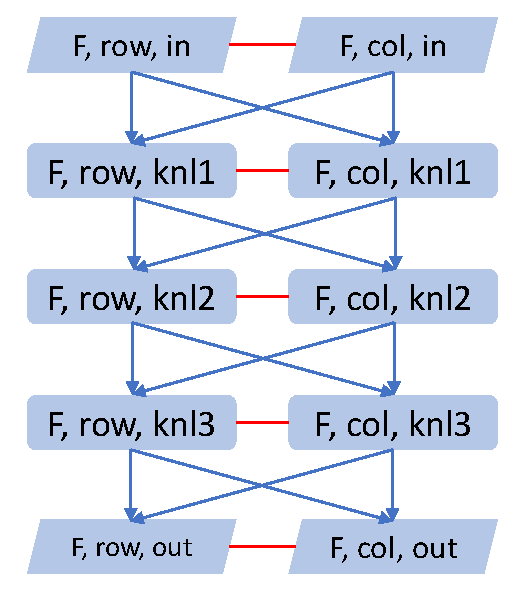
\includegraphics[page=1,width=\columnwidth]{ModelProgression.pdf}
		\caption{Initial state of the optimization problem.}\label{graphModel:1}
	\end{subfigure}
	\hspace{0.03\columnwidth}
	\begin{subfigure}[t]{0.3\columnwidth}
		\includegraphics[page=2,width=\columnwidth]{ModelProgression.pdf}
		\caption{After registering that F should be row-major during the second computation.}\label{graphModel:2}
	\end{subfigure}
	\hspace{0.03\columnwidth}
	\begin{subfigure}[t]{0.3\columnwidth}
		\includegraphics[page=3,width=\columnwidth]{ModelProgression.pdf}
		\caption{After registering that F should be column-major during the third computation.}\label{graphModel:3}
	\end{subfigure}
	
	\begin{subfigure}[t]{0.3\columnwidth}
		\includegraphics[page=4,width=\columnwidth]{ModelProgression.pdf}
		\caption{After the input format has been set and before the problem is solved. The model picks the output format and the format for knl1.}\label{graphModel:4}
	\end{subfigure}
	\hspace{0.03\columnwidth}
	\begin{subfigure}[t][0.15\columnwidth][b]{0.4\columnwidth}
		\begin{align*}
			x_{(F,row,in)} &+ x_{(F,col,in)} = 1 \\
			 \wedge \ x_{(F,row,knl1)} &+ x_{(F,col,knl1)} = 1 \\
			\wedge \ x_{(F,row,knl2)} &+ x_{(F,col,knl2)} = 1 \\
		  \wedge \ x_{(F,row,knl3)} &+ x_{(F,col,knl3)} = 1  \\
			\wedge \ x_{(F,row,out)} &+ x_{(F,col,out)} = 1 \\
			\wedge \ x_{(F,row,knl2)} = 1 \ &\wedge \ x_{(F,col,knl3)} = 1 \\
			\wedge \ x_{(F,row,in)}& = 1
		\end{align*}
		\caption{The algebraic representation of the constraints present when the problem is solved.}\label{graphModel:5}
	\end{subfigure}

	\caption{Graphical representation of the layout optimization problem for a View in \textsc{3mm}. Nodes represent possible format choices and edges represent format conversions. User choices constrain the possible paths through the graph.}\label{graphModel}
\end{figure}

\subsection{Constructing the Objective Function}

The objective function for the model estimates the runtime performance of different format choices by considering the costs of format uses and format conversions.

Each View reference in the computation contributes one term to the objective function for each possible data layout. This means that the reference \verb.F(i2,i1). in \verb.knl3.  contributes two terms.
The first term,  $c * x_{(F,row,knl3)}$,  represents the cost of that reference if \verb.F. were in row-major order. 
The second term, $c^\prime * x_{(F,col,knl3)}$  represents the cost of that reference if \verb.F. were in column-major order.
Because \verb.F. is not referenced in the first kernel, the objective function does not contain linear terms for either $x_{(F,row,knl1)}$ or $x_{(F,col,knl1)}$.
However, these decision variables appear in terms for format conversion costs.

Because a format conversion depends the format coming in and going out of the conversion, conversion cost terms contain two decision variables.
For example, consider the conversion step between \verb.knl1. and \verb.knl2..
There are two possible conversions to consider: row-major to row-major and column-major to row-major. 
Converting from row-major to row-major requires no action, so we  find the term $0 * x_{(F,row,knl1)} * x_{(F,row,knl2)}$ in the objective function.
Converting from column-major to row-major does require a reformatting, introducing the term $c^{\prime\prime} * x_{(F,col,knl1)} * x_{(F,row,knl2)}$.

Once the objective function is constructed, we can search for the format choices that minimize it, but first we need to determine the actual values for the cost coefficients.

\subsection{Determining Cost Coefficients}

It is generally possible to determine analytically if a kernel's data access would perform better with one layout or another; stride one accesses are preferable.
It is much more difficult to weigh the magnitude of this benefit against the cost of converting from one layout to another. 
Of course, there are useful heuristics, but model accuracy requires the incorporation of system-specific profiling information. 
Two types of costs need estimation: use costs, which represent the estimated cost of using a particular layout for a kernel, and conversion costs, which represent the cost of converting between formats.

Modeling the performance of a data access depends on three pieces of information: the nesting order of the kernel containing the access, the order of the dimensions in the View's layout, and the order of the arguments in the access.
Thus, the function we must construct to do this modeling will be parameterized by these attributes.
The nesting order is known at compile-time, as it is encoded in the kernel policy.
The access' argument order is gathered using RAJALC symbolic evaluation, so is not available until runtime.
Finally, because we are modeling the impact of using different layouts, this variable will also be changed at runtime.

Here, two related concerns emerge. 
First, because the profiling is executed at runtime, it is desirable to run as few profiling loops as possible to minimize overhead.
Second, because any modeling functions incorporated into RAJA are written and compiled before the runtime symbolic evaluation gathers the argument order, the modeling function cannot use the symbolic evaluation results to construct the profiling kernel. 
Instead, the profiling function must be constructed ahead of time to be capable of modeling an arbitrary access.
Thankfully, these problems can be addressed as a pair.
The approach here partitions the space of accesses, viewed as triples of the form $(nesting,layout,argument)$, into equivalence classes based on their expected performance characteristics.
Then, each equivalence class can be modeled using just one of its entries.

% plural bc me and the reader
Given a data access to classify, we begin by determining the nesting, layout, and argument orders.
The nesting order is found in the policy of the kernel containing the data access.
The values of the nesting order indicate which dimension of the iteration space each level of the loop nest will traverse. 
The argument order for a data access is the mapping between the dimensions of the iteration space and the dimensions of the data. 
For example, the argument order $(2,0)$ indicates that dimension 2 of the iteration space is used to index dimension 0 of the data, and that dimension 0 of the iteration space is used to index dimension 1 of the data.
Finally is the layout order, which is varied based on what layout the system is modeling. 
This ordering indicates the stride order of the dimensions.
For example, the layout order $(2,0,1)$ is stride-1 in the first dimension and has the largest stride in the second.

Figure~\ref{accessOrder} provides an overview of the classification process.

The first step is to normalize the argument order based on the layout order.
This process answers the question ``What argument order results in the same access pattern when using the canonical layout order?''
For example, consider the access $A(i_0,i_2,i_1)$ where $A$ has the layout order $(2,0,1)$ and the kernel has nesting order $(2,1,0)$.
If $A$ were to have the layout order $(0,1,2)$, what would the argument order need to be to have the same access pattern? 
If we permute the arguments by the layout order, we get our answer: $A(i_1, i_0, i_2)$.
So our layout-normalized argument order would be $(1,0,2)$. 

The second step is to normalize based on the kernel order. 
This process answers the question ``What argument order results in the same access pattern when using the canonical nesting order?''
This is done by identifying the position of each layout-normalized argument in the nesting order. 
Using the kernel order $(2,1,0)$ from above, We get a fully normalized access order of $(1,2,0)$.

All data accesses with the same fully normalized order are modelled using the same modeling kernel. 
This kernel is constructed with a fixed policy and argument order so that one lambda and kernel policy can be used for modeling each layout. 


\begin{figure*}
% chktex-file 44
\begin{subfigure}[b]{0.52\columnwidth}
\begin{lstlisting}
View2D A(a_data, rowMajor); 
View2D B(b_data, colMajor); 
View2D C(c_data, rowMajor);

auto mmLam = [&](auto i0, auto i1, auto i2) {
  C(i0,i1) += A(i0,i2) * B(i2,i1);
};
  
using Pol012 = KernelPolicy< 
  statement::For<0,loop_exec, // for i
	  statement::For<1,loop_exec, // for j
		  statement::For<2,loop_exec, // for k
			  statement::Lambda<0>
>>>>;
using Pol201 = KernelPolicy< 
	statement::For<2,loop_exec, // for k
		statement::For<0,loop_exec, // for i
			statement::For<1,loop_exec, // for j
				statement::Lambda<0>
>>>>;

auto knl1 = make_kernel<Pol012>(segs, mmLam);
auto knl2 = make_kernel<Pol201>(segs, mmLam);
\end{lstlisting}
\caption{Two kernels implementing matrix multiplication using different execution policies. The change in policy is equivalent to exchanging the loop nest order.}\label{accessOrder:code}
\end{subfigure}
\hspace{0.01\columnwidth}
	\begin{subfigure}[b]{0.45\columnwidth}
		\begin{center}
			\begin{tabular} {|c|c|c|}
\hline{}
Kernel & Nesting Order \\ \hline
knl1 & (0,1,2) \\
knl2 & (2,0,1) \\
\hline
			\end{tabular}

			\vspace{5px}

			\begin{tabular} {|c|c|c|}
				\hline 
				View & \makecell{Argument \\ Order} & \makecell{Layout \\ Order} \\  \hline 
				A & (0,2) & (0,1) \\ 
				B & (2,1) & (1,0) \\
				C & (0,1) & (0,1) \\
				\hline
			\end{tabular}

\vspace{5px}

			\begin{tabular} {|c|c|}
				\hline
				Information & Source \\ \hline 
				Argument Order & \makecell{Symbolic \\ evaluation}  \\ \hline
				Layout Order & \makecell{Varied for \\ modeling}\\ \hline
				Nesting Order & \makecell{Template \\parameter} \\
				\hline
			\end{tabular}
		\end{center}
		\caption{The information used to calculate access orders and how they are collected. Nesting orders come from the policies on lines 12--30, argument orders from the View references on line 9, and layout orders from the data initialization on lines 1--6.}\label{accessOrder:orders}
	\end{subfigure}

	\vspace{10px}

	\begin{subfigure}[b]{\columnwidth}
		\begin{center}
		Argument Order $\xrightarrow[\text{Layout Order}]{permute}$ Layout-Normalized Order

		Layout-Normalized Order $\xrightarrow[\text{Nesting Order}]{indexof}$ Access Order

%chktex-file 13
\begin{tabular}{c c}
		knl1, A: $(0,2)$ $\xrightarrow[(0,1)]{permute}$ $(0,2)$ $\xrightarrow[(0,1,2)]{indexof}$ $(0,2)$. & knl2, A: $(0,2)$ $\xrightarrow[(0,1)]{permute}$ $(2,0)$ $\xrightarrow[(2,0,1)]{indexof}$ $(0,1)$. \\
		knl1, B: $(2,1)$ $\xrightarrow[(1,0)]{permute}$ $(1,2)$ $\xrightarrow[(0,1,2)]{indexof}$ $(1,2)$. & knl2, B: $(2,1)$ $\xrightarrow[(1,0)]{permute}$ $(1,2)$ $\xrightarrow[(2,0,1)]{indexof}$ $(2,0)$. \\
		knl1, C: $(0,1)$ $\xrightarrow[(0,1)]{permute}$ $(0,1)$ $\xrightarrow[(0,1,2)]{indexof}$ $(0,1)$. & knl2, C: $(0,1)$ $\xrightarrow[(0,1)]{permute}$ $(0,1)$ $\xrightarrow[(2,0,1)]{indexof}$ $(1,2)$. \\
		
		
\end{tabular}
		\end{center}
	\caption{The calculation process. The first transformation normalizes different layouts. The second normalizes different nesting orders. The resulting tuple represents the canonical data access with the same performance behavior. References with the same access order can be modeled with the same microbenchmark.}\label{accessOrder:calc}
	\end{subfigure}

	
	\caption{Calculating access orders for the View references in two matrix multiplication kernels.~\ref{accessOrder:orders} shows the information extracted from~\ref{accessOrder:code}.~\ref{accessOrder:calc} shows how this information is used to estimate multiple reference costs with the same microbenchmark. }\label{accessOrder}

\end{figure*}



%%%%%%%%%%%%%%%%%%%%%%
\section{RAJAPerf Benchmark Suite}\label{sec:Experiment1}

The first evaluation experiment examines application performance and programmer productivity using benchmarks from the RAJA Performance Suite (RAJAPerf)~\cite{hornung2017raja}. 
When selecting benchmarks for inclusion in the evaluation, there are three criteria.
First, the benchmark needs to use multidimensional data. 
Benchmarks that use only scalar and one-dimensional data cannot be optimized with \FormatDecisions{} because there is only one format to choose from.
This criteria excludes 45 of the 63 benchmarks.
Second, the benchmark must make at least one access that traverses its data with a stride not equal to 1. 
Of the remaining 18, this excludes eight.
Finally, benchmarks with equal iteration space and data space dimensionality are excluded. 
This is to ensure enough data reuse to make conversion between formats worthwhile.
This leaves two matrix multiplication-based benchmarks and three partial assembly benchmarks.
However, because of the small extents in the partial assembly benchmarks, we focus on the \textsc{2mm} and \textsc{3mm} kernels.
To this pair, we add an additional four benchmarks to RAJAPerf's Polybench~\cite{pouchet2012polybench} section: \textsc{correlation}, \textsc{covariance}, \textsc{doitgen}, and \textsc{symm}. 

\textsc{2mm} solves the matrix expression $A*B*C$ using two matrix multiplications. 
First, it computes $A*B$ and stores the results in a temporary array.
Then this temporary result is multiplied by $C$.
\textsc{3mm} solves a similar matrix expression $A*B*C*D$ using three matrix multiplications.
It computes $A*B$, then $C*D$, then multiplies the results.
\textsc{correlation} and \textsc{covariance}, as the names suggest, calculate the correlation and covariance matrix for the input data. 
\textsc{correlation} has four loop nests and \textsc{covariance} has three.
\textsc{doitgen} is a multiresolution analysis kernel while \textsc{symm} computes a symmetric matrix-multiplication.

\begin{table}
	\centering
	%chktex-file 1
	%chktex-file 8
	\begin{tabular}{|c|c|c|c|c|}
		\hline
		Variant Name & Kernel Objects & Layout Changes & Chosen By & Written Using \\
		\hline
		\verb.RAJALC. & Yes & No & -- & -- \\
		\verb.Hand_Layout. & Yes & Yes & User & No API \\
		\verb.Format_Decisions. & Yes & Yes & User & API \\
		\verb.Model_Choice. & Yes & Yes & Model & API \\
		\hline
	\end{tabular}
	\caption{Benchmark variant descriptions.}\label{VariantDescription}
\end{table}
For each benchmark, I implement 4 variants and compare execution time and code length, shown in Table~\ref{VariantDescription}.
\verb.RAJALC. implements the computations using the kernel objects discussed is Section~\ref{sec:kernelObjects}. 
\verb.Hand_Layout. implements identified transformations without using \FormatDecisions. 
Because this variant does not have any analysis overhead, I expect this variant to be the fastest.
The \verb.Format_Decisions. variant uses \FormatDecisions to register the identified layout changes but does not use the model to look for other beneficial transformations.
Last, \verb.Model_Choice. allows the decision model to make all layout choices without providing any user-identified transformations.

\subsection{Performance Evaluation}\label{sec:systemDetails}
All performance results in this paper were collected on a single node with a 44-core IBM Power9 CPU and 256GB of CPU memory. 
I run with 22 threads on one socket to avoid transfers over a relatively slow inter-socket connection.
All compilation used GCC version 8.3.1 with \verb.-O3. optimization.
Figure~\ref{fig:speedups} reports the average speedup of the variants relative to the \verb.RAJALC. variant across 5 runs. 
I run the kernels at three problem sizes.
The default size for the RAJAPerf suite is SizeFactor=1, while SizeFactors 2 and 4 scale the problem size by 2 and 4, respectively.

\begin{figure*}
	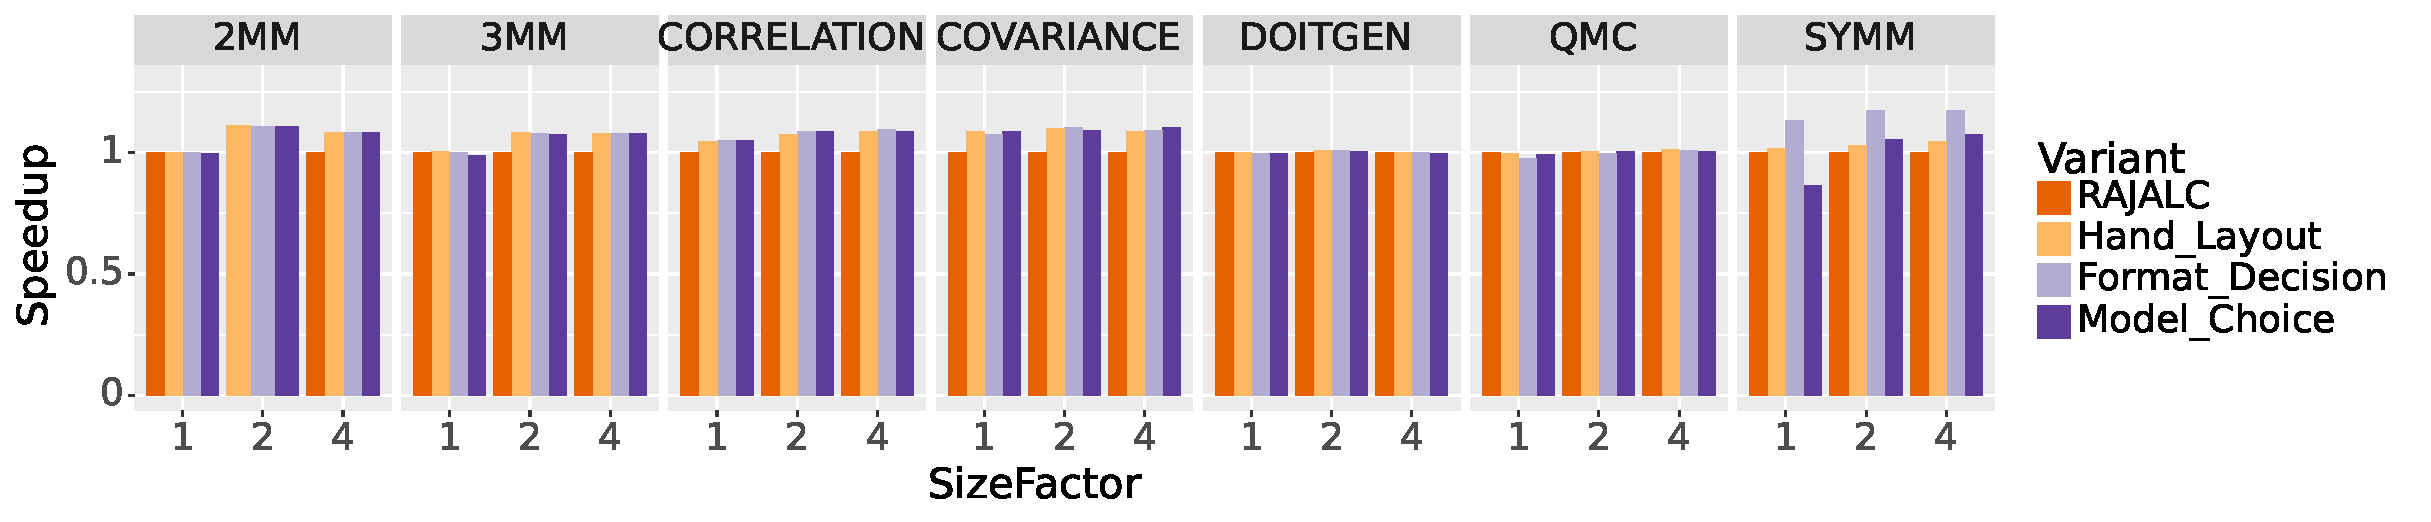
\includegraphics[width=0.9\textwidth]{speedups.pdf}
	\caption{Relative speedups of the different variants for different problem size factors. Speedup is calculated in reference to the RAJALC variant. Higher is better.}\label{fig:speedups}
\end{figure*}

For the \textsc{2mm} and \textsc{3mm} kernels, the performance of the three layout-changing variants are comparable. 
For the standard (SizeFactor=1) problem size, the performance effects are minimal, with \verb.Hand_Layout. providing a 0.3\% and 0.6\% speedup to \textsc{2mm} and \textsc{3mm} respectively. 
The \verb.Format_Decisions. variant provides a small 0.2\% speedup to \textsc{2mm} and 0.3\% to \textsc{3mm}, while the \verb.Model_Choice. variant shows a decrease in performance of 0.3\% and 1.3\%, respectively. 
With the middle problem size (SizeFactor=2), the performance effects of layout transformations are greater. 
For \textsc{2mm}, we see a 11.1\% speedup for the \verb.Hand_Layout. variant and 11.0\% for \verb.Format_Decisions. and \verb.Model_Choice. 
For \textsc{3mm}, we see a similar pattern slightly modified by the higher modeling costs of the \textsc{3mm} kernel. \verb.Hand_Layout. gives a 8.3\% speedup, \verb.Format_Decisions. a 8.1\% speedup, and \verb.Model_Choice. a 7.6\% speedup.
Finally, for the large problem size (SizeFactor=4), the results are similar.
All three variants of \textsc{2mm} see a 8.4\% speedup, whereas the variants of \textsc{3mm} see a 8.0\%, 7.9\%, and 7.8\% speedup.

For \textsc{correlation}, there is less variability across problem sizes. 
For SizeFactors 1, 2, and 4, the \verb.Hand_Layout. variant sees speedups of 4.6\%, 7.6\%, and 8.6\%, respectively. 
The \verb.Format_Decisions. variant does slightly better at 5.2\%, 8.6\%, and 9.6\%.
\verb.Model_Choice. remains competitive at 4.9\%, 8.6\%, and 8.7\%.
The \textsc{covariance} kernel performs similarly.
The \textsc{doitgen} kernel sees relatively flat performance across problem sizes and variants. All speedups are within 1.1\% of the baseline.

The \textsc{symm} kernel performs less consistently than the other kernels.
Still, the effects of the \verb.Hand_Layout. and \verb.Format_Decisions. variants share the same direction.
The standard problem size gives a 1.8\% speedup for \verb.Hand_Layout., a more significant speedup of 13.5\% for \verb.Format_Decisions., and a slowdown of 13.3\% for \verb.Model_Choice.. 
We attribute this slowdown for the standard problem size to the smaller amount of computation in the \textsc{symm} kernel that can offset the cost of the performance modeling. 
For SizeFactor=2, we see speedups across the board, at 3.2\%, 17.4\%, and 5.3\% respectively.
Finally, for SizeFactor=4, \verb.Hand_Layout. and \verb.Format_Decisions. give speedups of 4.6\% and 17.5\% while \verb.Model_Choice. gives a speedup of 7.5\%.


\subsection{Productivity Evaluation}

To evaluate the productivity of \FormatDecisions{}, I report the source lines of code added or changed for each of the variants.
This value is calculated by counting the number of line differences using python's \verb.Differ.. 
I preprocess to remove all whitespace-only lines.
Figure~\ref{PolybenchSLOC} shows the results.
With the exception of \textsc{3mm} and \textsc{qmc}, using \FormatDecisions{} requires between 2 and 3$\times$ fewer code changes than implementing the transformations by hand. 
When using the performance model to make the layout choices, this is reduced further, requiring 4 to 6$\times$ fewer code changes. 

While the productivity benefit here is significant, \FormatDecisions{} is especially useful when making subsequent layout changes after the first. 
Once a code has been changed to use \FormatDecisions{}, the change quantified in Figure~\ref{PolybenchSLOC}, further changes can be introduced with only a single line. 
For example, manually tuning data layouts for a new machine amounts to a handful of reordered characters to describe the new layouts, the second argument in the calls on lines 13-16 of Listing~\ref{FormatDecisions3MM}. 
Overall, by compressing the complexities of modifying data layouts, \FormatDecisions{} reduces the mental load on the programmer, freeing up capacity to explore more possible transformations.

\begin{figure}
	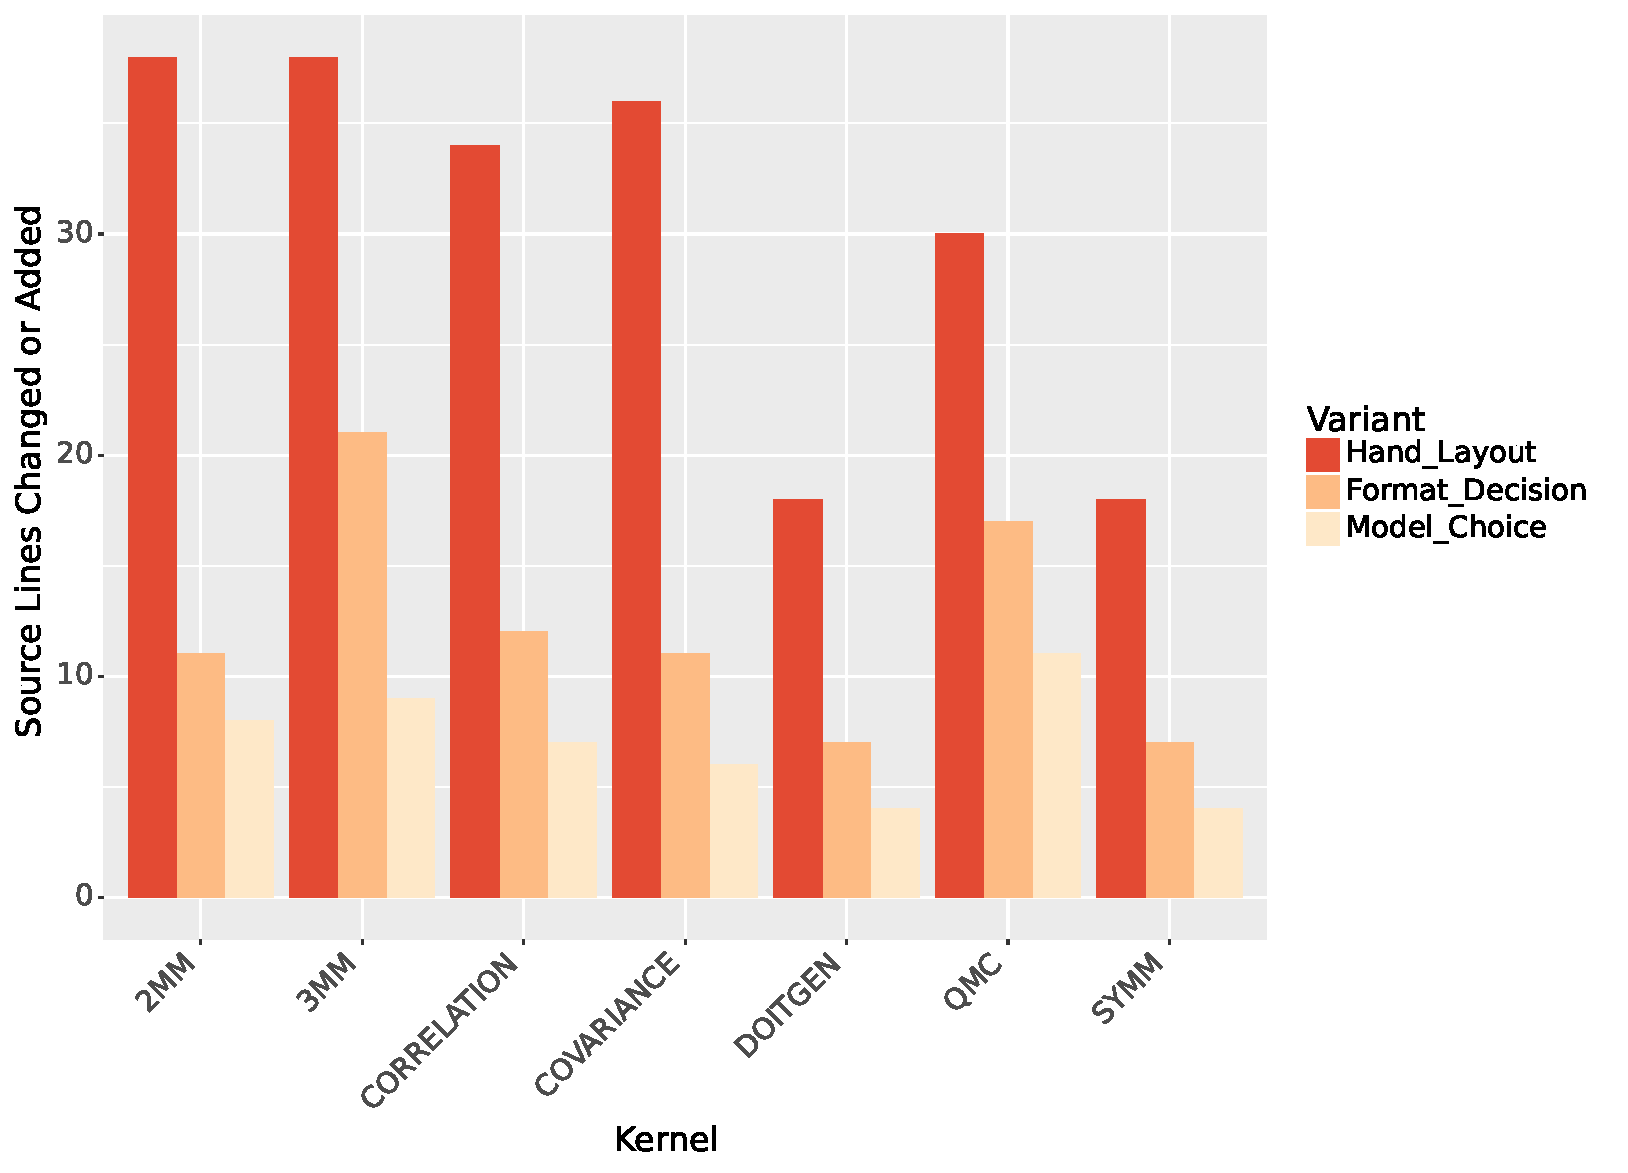
\includegraphics[width=\columnwidth]{sloc.pdf}
	\caption{Source lines of code modified (added, changed, or removed) relative to the  RAJALC variant. (Lower is better)}\label{PolybenchSLOC}  
\end{figure}

\section{Quantum Monte Carlo Simulation}\label{sec:miniQMC}
In all but the simplest (and least interesting) quantum systems, solving the Schr\"odinger equation requires numerical approximation. 
Quantum Monte Carlo algorithms have been developed as a solution to this problem of fast, accurate approximation.
QMCPACK~\cite{kim2018qmcpack} is one application implementing this approach, and lead to the development of a computationally representative miniapp, called miniQMC~\cite{richards2018fy18}.

As part of the evaluation of our contributions, we use \FormatDecisions{} to explore possible optimizations to miniQMC\@.
Intending to illustrate the progression of the exploration, we present a chronology of attempted transformations.
The results of our evaluation are mixed.
We identify layout transformations that improve performance compared to not making transformations, but it is overall slower than a version that immediately executes the kernel objects rather than grouping them in a container.
We show that this is due to the use of any containing object rather than any overhead caused by \FormatDecisions{} specifically.

\subsection{The Determinant Update Kernel}

\begin{figure}
\begin{lstlisting}[caption={Main loopchain of the determinant update kernel. Note that the access/storage order here is reversed.},label={updateInvMatRef}]
//tempMat = U^T * Ainv
for(i = 0; i < dc; i++) {
	for(j = 0; j < norb; j++) {
		tempMat(i,j) = 0;
		for(k = 0; k < norb; k++) {
			tempMat(j,i) += U(i,k) * Ainv(j,k);
		}
	}
}

for(i = 0; i < dc; i++) {
	tempMat(delay_list(i), i) -= 1;
}

//U = V * Binv
for(i = 0; i < dc; i++) {
	for(j = 0; j < norb; j++) {
		U(i,j) = 0;
		for(k = 0; k < norb; k++) {
			U(j,i) += V(k,i) * Binv(j,k);
		}
	}
}

// A -= U * tempMat
for(i = 0; i < dc; i++) {
	for(j = 0; j < norb; j++) {
		for(k = 0; k < norb; k++) {
			Ainv(j,i) -= U(k,i) * tempMat(j,k);
		}
	}
}
\end{lstlisting}
\end{figure}

miniQMC has four important kernels: determinant update, spline evaluation, Jastrow factors, and distance tables.
Of these, the determinant update kernel is most important, as it both accounts for 30 to 50\% of computation time and is the source of the application's cubic scaling.
The determinant update kernel is implemented by the \verb.DelayedUpdate. class.
This class maintains four matrices and two vectors internally and uses one passed as arguments to the methods. 
Once a sufficiently large number of updates have been collected, they are applied together with four loop nests.
First is the matrix multiplication $tempMat = U^{\top} * Ainv$.
Second is a one dimensional loop nest that updates $tempMat$.
Third is the matrix multiplication $U = V * Binv$.
Fourth and final is the matrix multiplication $Ainv -= U*tempMat$.
Listing~\ref{updateInvMatRef} shows a reference implementation for this loopchain.

A look at the second loop in the chain presents an early challenge: indirect accesses. 
\verb.tempMat. is indexed by the indirect access expression \verb.delay_list(i).. 
This type of access is not supported by the symbolic evaluation capabilities in RAJALC, meaning that the automated performance model cannot be used here.
However, this limitation does not restrict the programmer's ability to explore layout changes without the help of the performance model. 
For our experimentation, we use the `1 2 2'' shape, which simulates 128 atoms and 1536 electrons.

\subsection{Identifying Profitable Transformations}
\begin{figure}
\begin{lstlisting}[caption={Different layout transformations selected as part of the miniQMC exploration.}, label={miniQMCChoices}]
{ // RAJA baseline
	knl1(); //tempMat = U^T * Ainv
	knl2(); //tempMat(delay_list(i), i) -= 1;
	knl3(); //U = V * Binv
	knl4(); // A -= U * tempMat
}
{ // FormatDecisions baseline
	auto dec = format_decisions(tie(U,V,tempMat,Ainv), 
		knl1, knl2, knl3, knl4);
	auto comp = dec.generate();
	comp();
}
{// Fully enumerated version
	auto dec = format_decisions(tie(U,V,tempMat,Ainv), 
		knl1, knl2, knl3, knl4);
	dec.set_format_for(Ainv, {0,1}, knl1);
	dec.set_format_for(Ainv, {1,0}, knl4);
	dec.set_format_for(U, {0,1}, knl1);
	dec.set_format_for(U, {1,0}, knl3, knl4);
	dec.set_format_for(tempMat, {1,0}, knl1);
	dec.set_format_for(tempMat, {0,1}, knl4);
	dec.set_format_for(V, {1,0}, knl3);
	auto comp = dec.generate();
	comp();
}
{ // Refined version
auto dec = format_decisions(tie(U,V), 
knl1, knl2, knl3, knl4);
dec.set_format_for(U, {0,1}, knl1);
dec.set_format_for(U, {1,0}, knl3, knl4);
dec.set_format_for(V, {1,0}, knl3);
auto comp = dec.generate();
comp();
}
\end{lstlisting}
\end{figure}

To begin the search for a profitable transformation sequence, I enumerate the accesses with orders that do not align with the schedule, transforming to a layout with a stride of one.
These selections can be seen in Figure~\ref{miniQMCChoices}
However, this complete enumeration is slower than a baseline \FormatDecisions{} version that makes no conversions at all, with a runtime of 27.28 seconds compared to the baseline's 23.63.

To refine the transformation sequence, we note that the access to \verb.Ainv. in the final kernel does not change most iterations, as it does not use the innermost loop index. 
The second transformation sequence uses this fact, making format choices only on Views that use the innermost index. 
This version executes in 22.38 seconds, an improvement over the \FormatDecisions{} baseline. 
Subsequent versions transforming only \verb.U. or \verb.V. indicate that this performance improvement is coming mainly from the transformations to \verb.U.

\subsection{Proving Constness}

While I am able to identify a transformation sequence that improves performance compared to the \FormatDecisions{} baseline, there is significant performance overhead compared to the RAJA baseline, 23.63 and 10.18 seconds respectively.
The first possible cause to explore is overhead from initializing the \FormatDecisions{} object, registering transformations, and generating the final computation. 
To explore this hypothesis, I return to the baseline implementation and wrap these components in an additional timer. 
However, this timer clocks a vanishingly small contribution: 0.0022 seconds.

If the overhead is not a product of the \FormatDecisions{} object itself, it must be from the computation object it generates.
Regardless of what conversions are registered, this computation object is a fixed-length loop chain.
Between each of the kernels from the computation itself is one converter kernel for each of the Views being considered as targets for conversions.
When there are no conversions to make, these converters should quickly resolve to a no-op.
To better understand their contribution to the overall execution time, I compare the baseline, which has four converters between each of the original kernels, with a version that has just one.
Compared to the baseline's 23.63 seconds, this version takes 23.43.
While an ever-so-slight reduction in execution time, it is not nearly enough to account for the overhead.

With the converters eliminated as a suspect, I am left only with the kernel container that holds the loop chain.
I can create this container manually to exclude any possible influence of the \FormatDecisions{} code.
With an execution that takes 23.50 seconds, there is a clue as to the underlying cause.
Something about having the kernel objects in a container is affecting their performance.
At first glance, it seems that something in the chain's execution is causing the problem.
However, this is unlikely, as the chain's call operator resolves at compile time to just a sequence of calls to each of the kernels.

I can confirm this with a version that creates the loop chain object, but does not use it to run the computation.
This version takes 23.44 seconds, even though it, like the faster RAJA baseline, executes the kernel directly.
This suggests that important compiler optimizations are no longer applied when the kernel objects are incorporated into another object. 
However, when constructed with const references rather than by value, this performance reduction is removed.

\section{Related Work}

Early approaches to optimizing data locality use schedule transformations rather than data layout transformations. 
Work incorporated into the SUIF compiler uses interchange, reversal, skewing, and tiling~\cite{wolf1991data}, whereas Fortran source-to-source approaches also use loop fusion~\cite{mckinley1996improving}.
While schedule transformations avoid the overhead cost of layout conversion, their global nature can improve locality for one access while harming another.
Nevertheless, schedule transformations remain a popular approach to optimizing data locality and parallelism, 
especially through tiling techniques~\cite{bondhugula2008pluto,bertolacci2015parameterized,bondhugula2016diamond,bandishti2012tiling,unat2016tida}.

In the domain of data layout transformations, early work in High Performance Fortran (HPF) and D compilers~\cite{bixby1994automatic,kennedy1995automatic,kennedy1998automatic} provide foundations for a variety of later approaches.
Their framework follows a popular pattern: generate a space of possible choices, estimate the performance of different choices, and select an option using an ILP formulation. 
The problem formulation used here is similar to theirs, although we do not use the data layout graph intermediate representation.
Furthermore, where their model for cost estimation focuses on communication costs in a distributed context, our approach models on-node performance costs of cache misses.

The polyhedral model, traditionally used for schedule transformations, is commonly leveraged for data layout transformations as well.
With the rise of multicore chips, new strategies were needed to manage shared on-chip resources. 
Work by Lu et al.~\cite{lu2009data} and Zhang et al.~\cite{zhang2011optimizing} develop layout optimization schemes based on the polyhedral model and use a combination of strip-mining, permutation, and padding transformations.


Data layout transformation frameworks are also popular for heterogeneous programming systems, especially for stencil codes.
Sung, Stratton, and Hwu~\cite{sung2010data} use data layout transformations to relieve pressure on memory controllers in structured grid applications by spreading data out across the address space based on the indexing behavior of the application.
Henretty et al.~\cite{henretty2011data} develop a layout transformation and accompanying static analysis to address stream alignment conflicts for SIMD architectures.
Jaeger and Barthou~\cite{jaeger2012automatic} present a strategy for generating stencil codes with optimal data layouts using a multi-padding layout transformation.
Recognizing the need for specialized support for ever-changing chip structure, Majeti et al.~\cite{majeti2013compiler} develop a programmer (or autotuner) guided data transformation system.
Built into the Habenero-C compiler, the meta-data provided by the user guides the generation of architecture-specific SOA, AOS, and SOAOS data layouts.
Another approach by Kofler, Cosenza, and Fahringer~\cite{kofler2015automatic} convert AOS implementations to other data layouts for GPU applications automatically.  
With the exception of Majeti et al., these approaches do not provide an interface to the developer, and without exception are compiler-based approaches.
The \FormatDecisions{} approach presents an interface to the developer in the form of a library API, allowing user control and low-cost integration into existing workloads.

Although still in the realm of the compiler-based techniques, pragmas have been suggested as a solution to the problem of providing control over the transformations to the user.
Proposals to add such pragmas have been submitted to OpenMP~\cite{kruse2019design} and Clang~\cite{kruse2018user}.
Other work has implemented transformation pragmas into a source-to-source compiler~\cite{xu2014semi}. 


Domain-specific language approaches are another avenue for presenting users with control of the data layout transformations to apply. 
Kronawitter et al.~\cite{kronawitter2018automatic} incorporate data layout specifications into the ExaSlang DSL.
Using a polyhedral framework, the Tiramisu DSL~\cite{baghdadi2019tiramisu} also enables data layout transformation specifications.
In contrast to these specialized approaches, our approach seeks to support a wider class of computations without needing the additional machinery required to use DSLs. 


\section{Conclusion}


Effective use of the memory hierarchy is critical to application performance.
One way of doing this is by changing how data is stored within memory.
Yet, in performance portability libraries like RAJA and Kokkos, where one codebase is used for machines with different architectures, there are not yet tools for transforming the layout of data between parts of a computation. 
Thus, if a developer wants to introduce these optimizations, they are left in a time-consuming, error-prone situation --- further exacerbated by the potential for data layout transformations to not be worth the overhead.

This chapter's contribution, \FormatDecisions, remedies this situation by combining declarative format specification  interface with runtime performance modeling to supplement user directives.
Integrated directly into the performance portability library RAJA, but possible in any library with computation objects and a data View-like abstraction, \FormatDecisions{} provides a flexible interface for quick exploration of data layout changes. 
Additionally, \FormatDecisions{} uses an ILP formulation to optionally identify other profitable transformations, \enquote{filling in} the user specification.

When evaluated against hand-implemented layout transformations on seven benchmark kernels, \FormatDecisions{} provides comparable performance improvements with a fraction of the code changes.
Furthermore, subsequent modifications to the layout transformations, for example as part of porting a codebase to a new machine, are reduced to single-line changes. 
This improves maintainability and reduces the potential for introducing bugs.
Overall, by approaching data layout optimization from the direction of programmer productivity, \FormatDecisions{} enables developers to explore different layouts with ease. 



\begin{comment}
\section{3D Partial Assembly}

The kernel \verb.MASS3DPA. is notable for its complex nestings and chain length. 
Within the outermost loop, it allocates two cubes, \verb.sm0. and \verb.sm1., of side length \verb.MDQ..
There are five persistent allocations: \verb.B., \verb.Bt., \verb.D., \verb.X., and \verb.Y.. 
\verb.B. and \verb.Bt. are two dimensional, while the others are four. 
\verb.Y. is the output value.
\verb.MQ1. is set to 5, and \verb.MD1. to 4. 


\begin{lstlisting}[caption={3D Mass Partial Assembly reference implementation}]
for e in 0..< NE {
	//DDQ <- X
	for (dy, qx, dx, dz) in (0,0,0,0)..<(D1D, Q1D, D1D, D1D) {
		DDQ(dz, dy, qx) += X(dx, dy, dz, e) * Btsmem(qx, dx);
	}

	//DQQ <- DDQ
	for (qy, qx, dy, dz) in (0,0,0,0)..<(Q1D, Q1D, D1D, D1D) {
		DQQ(dz, qy, qx) += DDQ(dz, dy, qx) * Btsmem(qy, dy);
	}

	//QQQ <- DQQ and D
	for (dy, qx, dz, qz) in (0,0,0,0)..<(Q1D, Q1D, D1D, Q1D) {
		QQQ(qz, qy, qx) += DQQ(dz, qy, qx) * Bsmem(qz, dz) * D(qx, qy, qz, e);
	}

	for (d,q) in (0,0)..<(D1D, Q1D) {
		Btsmem(d,q) = Bt(q,d);
	}

	//QQD <- QQQ
	for (qy, dx, qx, qz) in (0,0,0,0)..<(Q1D, D1D, Q1D, Q1D) {
		QQD(qz, qy, dx) += QQQ(qz, qy, qx) * Btsmem(dx, qx);
	}

	// QDD <- QQD
	for (dy, dx, qy, qz) in (0,0,0,0)..<(D1D, D1D, Q1D, Q1D) {
		QDD(qz, dy, dx) += QQD(qz, qy, dx) * Btsmem(dy, qy);
	}

	// Y <- QDD
	for (dy,dx,qz,dz) in (0,0,0,0)..<(D1D, D1D, Q1D, D1D) {
		Y(dx, dy, dz, e) += QDD(qz, dy, dx) * Btsmem(dz, qz);
	}
}

\end{lstlisting}

Overall, we go from an array of DDD (X), to an array of DDD (Y), trading one dimension at a time from D to Q, then back. DDD -> QQQ -> DDD. This is facilitated by the B array, which is addressed by the d and q dimensions of each of x, y, and z. 
As we reach QQQ, we also multiply in D, then flip B's memory to convert back from Q to D.

Xsmem is, at the beginning of each loop, assigned to a 3D hyperslice of the 4D \verb.X. structure.
Each of the 3 dimensional structures, DDQ, DQQ, QQQ, QQD, and QDD, are temporaries that share the two cubed data structures. 
Furthermore, all loops except for the one transposing \verb.Bt. are implemented using a temporary vector \verb.u. to accumulate the updates.

To implement this kernel and explore its optimization, we begin with a version without the various temporary storage optimizations. 
This means we give the temporary Views their own storage and accumulate directly into the multidimensional arrays rather than using a temporary vector.

Additionally, to not clobber the existing port in RAJAPerf, we use lowercase variable names for teh views.
	
\end{comment}
